% Options for packages loaded elsewhere
\PassOptionsToPackage{unicode}{hyperref}
\PassOptionsToPackage{hyphens}{url}
\PassOptionsToPackage{dvipsnames,svgnames,x11names}{xcolor}
%
\documentclass[
  12pt]{article}

\usepackage{amsmath,amssymb}
\usepackage{iftex}
\ifPDFTeX
  \usepackage[T1]{fontenc}
  \usepackage[utf8]{inputenc}
  \usepackage{textcomp} % provide euro and other symbols
\else % if luatex or xetex
  \usepackage{unicode-math}
  \defaultfontfeatures{Scale=MatchLowercase}
  \defaultfontfeatures[\rmfamily]{Ligatures=TeX,Scale=1}
\fi
\usepackage{lmodern}
\ifPDFTeX\else  
    % xetex/luatex font selection
\fi
% Use upquote if available, for straight quotes in verbatim environments
\IfFileExists{upquote.sty}{\usepackage{upquote}}{}
\IfFileExists{microtype.sty}{% use microtype if available
  \usepackage[]{microtype}
  \UseMicrotypeSet[protrusion]{basicmath} % disable protrusion for tt fonts
}{}
\makeatletter
\@ifundefined{KOMAClassName}{% if non-KOMA class
  \IfFileExists{parskip.sty}{%
    \usepackage{parskip}
  }{% else
    \setlength{\parindent}{0pt}
    \setlength{\parskip}{6pt plus 2pt minus 1pt}}
}{% if KOMA class
  \KOMAoptions{parskip=half}}
\makeatother
\usepackage{xcolor}
\setlength{\emergencystretch}{3em} % prevent overfull lines
\setcounter{secnumdepth}{5}
% Make \paragraph and \subparagraph free-standing
\makeatletter
\ifx\paragraph\undefined\else
  \let\oldparagraph\paragraph
  \renewcommand{\paragraph}{
    \@ifstar
      \xxxParagraphStar
      \xxxParagraphNoStar
  }
  \newcommand{\xxxParagraphStar}[1]{\oldparagraph*{#1}\mbox{}}
  \newcommand{\xxxParagraphNoStar}[1]{\oldparagraph{#1}\mbox{}}
\fi
\ifx\subparagraph\undefined\else
  \let\oldsubparagraph\subparagraph
  \renewcommand{\subparagraph}{
    \@ifstar
      \xxxSubParagraphStar
      \xxxSubParagraphNoStar
  }
  \newcommand{\xxxSubParagraphStar}[1]{\oldsubparagraph*{#1}\mbox{}}
  \newcommand{\xxxSubParagraphNoStar}[1]{\oldsubparagraph{#1}\mbox{}}
\fi
\makeatother


\providecommand{\tightlist}{%
  \setlength{\itemsep}{0pt}\setlength{\parskip}{0pt}}\usepackage{longtable,booktabs,array}
\usepackage{calc} % for calculating minipage widths
% Correct order of tables after \paragraph or \subparagraph
\usepackage{etoolbox}
\makeatletter
\patchcmd\longtable{\par}{\if@noskipsec\mbox{}\fi\par}{}{}
\makeatother
% Allow footnotes in longtable head/foot
\IfFileExists{footnotehyper.sty}{\usepackage{footnotehyper}}{\usepackage{footnote}}
\makesavenoteenv{longtable}
\usepackage{graphicx}
\makeatletter
\newsavebox\pandoc@box
\newcommand*\pandocbounded[1]{% scales image to fit in text height/width
  \sbox\pandoc@box{#1}%
  \Gscale@div\@tempa{\textheight}{\dimexpr\ht\pandoc@box+\dp\pandoc@box\relax}%
  \Gscale@div\@tempb{\linewidth}{\wd\pandoc@box}%
  \ifdim\@tempb\p@<\@tempa\p@\let\@tempa\@tempb\fi% select the smaller of both
  \ifdim\@tempa\p@<\p@\scalebox{\@tempa}{\usebox\pandoc@box}%
  \else\usebox{\pandoc@box}%
  \fi%
}
% Set default figure placement to htbp
\def\fps@figure{htbp}
\makeatother

\addtolength{\oddsidemargin}{-.5in}%
\addtolength{\evensidemargin}{-1in}%
\addtolength{\textwidth}{1in}%
\addtolength{\textheight}{1.7in}%
\addtolength{\topmargin}{-1in}%
\usepackage{booktabs}
\usepackage{longtable}
\usepackage{array}
\usepackage{multirow}
\usepackage{wrapfig}
\usepackage{float}
\usepackage{colortbl}
\usepackage{pdflscape}
\usepackage{tabu}
\usepackage{threeparttable}
\usepackage{threeparttablex}
\usepackage[normalem]{ulem}
\usepackage{makecell}
\usepackage{xcolor}
\usepackage{amsmath}
\usepackage{float}
\usepackage{hyperref}
\usepackage[utf8]{inputenc}
\usepackage{bm}
\def\tightlist{}
\usepackage{setspace}
\newcommand\pD{$p\text{-}D$}
\newcommand\kD{$k\text{-}D$}
\newcommand\dD{$d\text{-}D$}
\newcommand\gD{$2\text{-}D$}
\newcommand{\To}{\textbf{to}~}
\usepackage{abstract}
\renewcommand{\abstractname}{}    % clear the title
\renewcommand{\absnamepos}{empty} % originally center
\makeatletter
\@ifpackageloaded{caption}{}{\usepackage{caption}}
\AtBeginDocument{%
\ifdefined\contentsname
  \renewcommand*\contentsname{Table of contents}
\else
  \newcommand\contentsname{Table of contents}
\fi
\ifdefined\listfigurename
  \renewcommand*\listfigurename{List of Figures}
\else
  \newcommand\listfigurename{List of Figures}
\fi
\ifdefined\listtablename
  \renewcommand*\listtablename{List of Tables}
\else
  \newcommand\listtablename{List of Tables}
\fi
\ifdefined\figurename
  \renewcommand*\figurename{Figure}
\else
  \newcommand\figurename{Figure}
\fi
\ifdefined\tablename
  \renewcommand*\tablename{Table}
\else
  \newcommand\tablename{Table}
\fi
}
\@ifpackageloaded{float}{}{\usepackage{float}}
\floatstyle{ruled}
\@ifundefined{c@chapter}{\newfloat{codelisting}{h}{lop}}{\newfloat{codelisting}{h}{lop}[chapter]}
\floatname{codelisting}{Listing}
\newcommand*\listoflistings{\listof{codelisting}{List of Listings}}
\makeatother
\makeatletter
\makeatother
\makeatletter
\@ifpackageloaded{caption}{}{\usepackage{caption}}
\@ifpackageloaded{subcaption}{}{\usepackage{subcaption}}
\makeatother

\usepackage[]{natbib}
\bibliographystyle{agsm}
\usepackage{bookmark}

\IfFileExists{xurl.sty}{\usepackage{xurl}}{} % add URL line breaks if available
\urlstyle{same} % disable monospaced font for URLs
\hypersetup{
  pdftitle={Appendix: Looking at Non-Linear Dimension Reductions as Models in the Data Space},
  pdfauthor={Jayani P. Gamage; Dianne Cook; Paul Harrison; Michael Lydeamore; Thiyanga S. Talagala},
  colorlinks=true,
  linkcolor={blue},
  filecolor={Maroon},
  citecolor={Blue},
  urlcolor={Blue},
  pdfcreator={LaTeX via pandoc}}



\begin{document}


\def\spacingset#1{\renewcommand{\baselinestretch}%
{#1}\small\normalsize} \spacingset{1}


%%%%%%%%%%%%%%%%%%%%%%%%%%%%%%%%%%%%%%%%%%%%%%%%%%%%%%%%%%%%%%%%%%%%%%%%%%%%%%

\title{\bf Appendix: Looking at Non-Linear Dimension Reductions as
Models in the Data Space}
\author{
Jayani P. Gamage\\
Econometrics \& Business Statistics, Monash University\\
and\\Dianne Cook\\
Econometrics \& Business Statistics, Monash University\\
and\\Paul Harrison\\
MGBP, BDInstitute, Monash University\\
and\\Michael Lydeamore\\
Econometrics \& Business Statistics, Monash University\\
and\\Thiyanga S. Talagala\\
Statistics, University of Sri Jayewardenepura\\
}
\maketitle

\bigskip
\bigskip
\begin{abstract}

\end{abstract}


\newpage
\spacingset{1.9} % DON'T change the spacing!


\begin{table}

\centering{

\centering\begingroup\fontsize{12}{14}\selectfont

\begin{tabular}{>{\raggedright\arraybackslash}p{3cm}>{\raggedright\arraybackslash}p{12cm}}
\toprule
\textbf{Notation} & \textbf{Description}\\
\midrule
$n, p, k$ & number of observations, variables, embedding dimension, respectively\\
$\mathbfit{X}, \mathbfit{x}$ & $p$-dimensional data (population, sample)\\
$\mathbfit{y}$ & $k$-dimensional layout\\
$P$ & orthonormal basis, generating a $d\text{-}dimensional$ linear projection of $p$-dimensional data\\
$T$ & true  model\\
\addlinespace
$g$ & functional mapping from \pD{} to \kD{}, especially as prescribed by NLDR\\
$\mathbfit{\theta}$ & (Hyper-) parameters for NLDR method\\
$r$ & ranges of the embedding components\\
$C^{(j)}$ & $j$-dimensional bin centers\\
$(b_1, b_2)$ & number of bins in each direction\\
\addlinespace
$(a_1, a_2)$ & binwidths, distance between centroids in each direction\\
$(s_1, \ s_2)$ & starting coordinates of the hexagonal grid\\
$q$ & buffer to ensure hexgrid covers data, proportion of data range, 0-1\\
$m$ & number of non-empty bins\\
$b$ & number of  hexagons in the grid\\
\addlinespace
$h$ & hexagonal id\\
$l$ & side length\\
$A$ & area\\
\bottomrule
\end{tabular}
\endgroup{}

}

\caption{\label{tbl-notation}Summary of notation for describing new
methodology.}

\end{table}%

\newpage

\section{Computing hexagon grid
configurations}\label{computing-hexagon-grid-configurations}

Given range of embedding component, \(r_2\), number of bins along the
x-axis, \(b_1\), and buffer proportion, \(q\), hexagonal starting point
coordinates, \(s_1 = -q\), and \(s_2 = -q \times r_2\). The purpose is
to find width of the hexagon. \(a_1\), and number of bins along the
y-axis, \(b_2\).

\begin{figure}[H]

\centering{

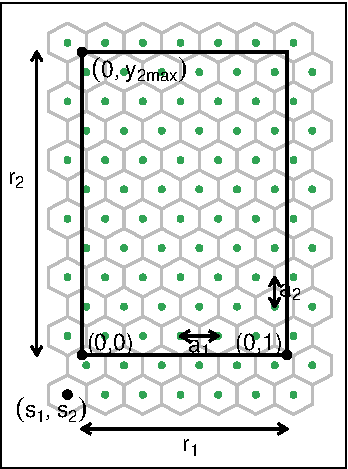
\includegraphics[width=0.3\linewidth,height=\textheight,keepaspectratio]{appendix_files/figure-pdf/fig-hex-param-1.pdf}

}

\caption{\label{fig-hex-param}The components of the hexagon grid
illustrating notation.}

\end{figure}%

Geometric arguments give rise to the following constraints.

\(\text{min }a_1 \text{ s.t.}\)

\begin{equation}\phantomsection\label{eq-equation1}{
s_1 - \frac{a_1}{2} < 0,
}\end{equation}

\begin{equation}\phantomsection\label{eq-equation2}{
s_1 + (b_1 - 1) \times a_1 > 1,
}\end{equation}

\begin{equation}\phantomsection\label{eq-equation4}{
s_2 - \frac{a_2}{2} < 0,
}\end{equation}

\begin{equation}\phantomsection\label{eq-equation5}{
s_2 + (b_2 - 1) \times a_2 > r_2.
}\end{equation}

Since \(a_1\) and \(a_2\) are distances,

\[
a_1, a_2 > 0.
\] Also, \((s_1, s_2) \in (-0.1, -0.05)\) as these are multiplicative
offsets in the negative direction.

Equation~\ref{eq-equation1} can be rearranged as,

\[
a_1 > 2s_1
\]

which given \(s_1 < 0\) and \(a_1 > 0\) will \emph{always} be true. The
same logic follows for Equation~\ref{eq-equation4} and substituting
\(a_2 = \frac{\sqrt{3}}{2}a_1\), and \(s_2 = -q \times r_2\) to
Equation~\ref{eq-equation4} can be written as,

\[
a_1 > -\frac{4}{\sqrt{3}}qr_2
\]

Also, substituting \(a_2 = \frac{\sqrt{3}}{2}a_1\),
\(s_2 = -q \times r_2\) and rearranging Equation~\ref{eq-equation5}
gives:

\begin{equation}\phantomsection\label{eq-equation6}{
a_1 > \frac{2(r_2 + qr_2)}{\sqrt{3}(b_2 - 1)}.
}\end{equation}

Similarly, substituting \(s_1 = -q\) Equation~\ref{eq-equation2}
becomes,

\begin{equation}\phantomsection\label{eq-equation7}{
a_1 > \frac{(1 + q)}{(b_1 - 1)}.
}\end{equation}

This is a linear optimization problem. Therefore, the optimal solution
must occur on a vertex. So, by setting Equation~\ref{eq-equation6}
equals to Equation~\ref{eq-equation7} gives,

\[
\frac{2(r_2 + qr_2)}{\sqrt{3}(b_2 - 1)} = \frac{(1 + q)}{(b_1 - 1)}.
\]

After rearranging this,

\[
b_2 = 1 + \frac{2r_2(b_1 - 1)}{\sqrt{3}}
\]

and since \(b_2\) should be an integer,

\begin{equation}\phantomsection\label{eq-equation8}{
b_2 = \Big\lceil1 +\frac{2r_2(b_1 - 1)}{\sqrt{3}}\Big\rceil.
}\end{equation}

Furthermore, with known \(b_1\) and \(b_2\), by considering
Equation~\ref{eq-equation2} or Equation~\ref{eq-equation5} as the
\emph{binding} or \emph{active constraint}, can compute \(a_1\).

If Equation~\ref{eq-equation2} is active, then,

\[
\frac{(1 + q)}{(b_1 - 1)} < \frac{2(r_2 + qr_2)}{\sqrt{3}(b_2 - 1)}.
\]

Rearranging this gives,

\[
r_2 > \frac{\sqrt{3}(b_2 - 1)}{2(b_1 - 1)}.
\]

Therefore, if this equality is true, then
\(a_1 = \frac{(1+q)}{(b_1 - 1)}\), otherwise,
\(a_1 = \frac{2r_2(1+q)}{\sqrt{3}(b_2 - 1)}\).

\newpage

\section{Binning the data}\label{binning-the-data}

Points are assigned to the bin they fall into based on the nearest
centroid. If a point is equidistant from multiple centroids, it is
assigned to the centroid with the lowest hexagonal bin ID.

\begin{figure}

\centering{

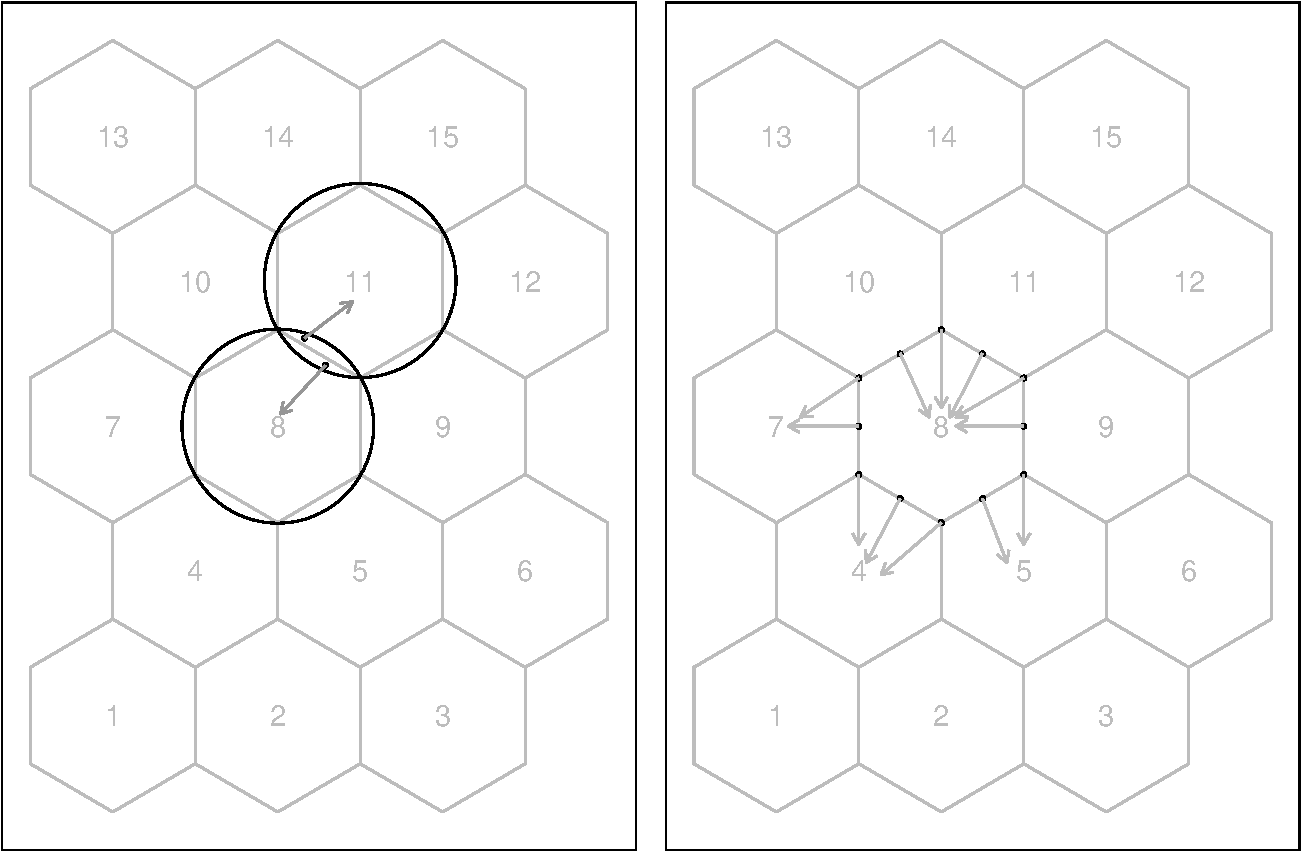
\includegraphics[width=1\linewidth,height=\textheight,keepaspectratio]{appendix_files/figure-pdf/fig-assign-data-1.pdf}

}

\caption{\label{fig-assign-data}Binning the data. Points are assigned to
the nearest centroid. If a point is equidistant from multiple centroids,
assigned to the lowest centroid.}

\end{figure}%

\newpage

\section{Area of a hexagon}\label{area-of-a-hexagon}

The area of a hexagon is defined as \(A = \frac{3\sqrt{3}}{2}l^2\),
where \(l\) is the side length of the hexagon. \(l\) can be computed
using \(a_1\) and \(a_2\).

\begin{figure}

\centering{

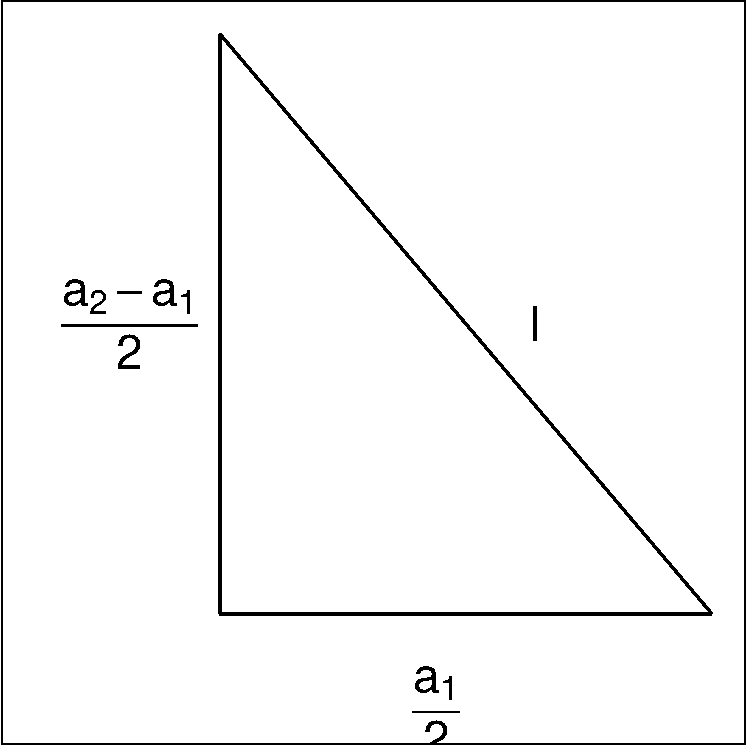
\includegraphics[width=0.3\linewidth,height=\textheight,keepaspectratio]{appendix_files/figure-pdf/fig-tri-param-1.pdf}

}

\caption{\label{fig-tri-param}The components of the right triangle
illustrating notation.}

\end{figure}%

By applying the Pythagorean theorem, we obtain,

\[
l^2 = \left(\frac{a_1}{2}\right)^2 + \left(\frac{a_2 - l}{2}\right)^2.
\] Next, rearranging the terms, we get,

\[
l^2 - \left(\frac{a_2 - l}{2}\right)^2 = \left(\frac{a_1}{2}\right)^2,
\]

\[
\left[l - \left(\frac{a_2 - l}{2}\right)\right]\left[l + \left(\frac{a_2 - l}{2}\right)\right] = \left(\frac{a_1}{2}\right)^2,
\]

\[
3l^2 + 2a_2l - (a_1^2 + a_2^2) = 0.
\]

Finally, by solving the quadratic equation, we compute,

\[
l = \frac{-2a_2 \pm \sqrt{4a_2^2 - 24[-(a_1^2 + a_2^2)]}}{6},
\]

\[
l = \frac{-a_2 \pm \sqrt{a_2^2 - 6[-(a_1^2 + a_2^2)]}}{3},
\]

where \(l > 0\).

\section{Single-cell gene expression: comparison with results of scDEED
recommendations}\label{single-cell-gene-expression-comparison-with-results-of-scdeed-recommendations}

As we were writing this paper \citet{xia2023} appeared proposing a new
method called scDEED helping to assess the validity of a \gD{}
embedding. scDEED calculates a reliability score for each cell embedding
based on the similarity between the cell's \gD{} embedding neighbors and
its neighbors prior to embedding. A low reliability score suggests a
dubious embedding. It can help in the deciding on optimal
hyper-parameters. Here we illustrate how our method compares with the
results from scDEED.

Following the process in \citet{xia2023} again using the Human
Peripheral Blood Mononuclear Cells (PBMC) data. Note that
\citet{xia2023} uses a different subset from the PBMC dataset used by
\citet{chen2024}, which contains \(31,021\) cells including cell type
labels, and the gene expression levels were in the unit of
log-transformed UMI count per \(10,000\). They focused on three
sequencing methods (inDrops, DropSeq, and SeqWell) and four common cell
types Cytotoxic T cell, CD4+T cell, CD14+ Monocyte, and B cell.

For illustration purposes, we only selected cells generated with inDrops
(\(n=5858\) cells) and UMAP and tSNE cell embeddings. Also,
\citet{xia2023} used first \(9\) principal components to generate the
UMAP and tSNE. The objective is to assess the optimized layout by
scDEED, and if it does not accurately represent the three clusters with
small separations of the PBMC dataset, then select a reasonable \gD{}
layout.

The layout a (Figure~\ref{fig-pbmc-mse-umap}) is generated from the
hyper-parameters suggested by \citet{chen2023}, and the layout b
(Figure~\ref{fig-pbmc-mse-umap}) is with suggested hyper-parameters by
scDEED to be more accurate. The layout a and b contain \(46\) and \(83\)
dubious cells respectively.

The log MSE vs binwidth (\(a_1\)) plot (Figure~\ref{fig-pbmc-mse-umap})
illustrates that our approach would suggest that scDEED is correct here,
that layout b is more accurately reflecting the cluster structure in the
PBMC data.

\begin{figure}[H]

\centering{

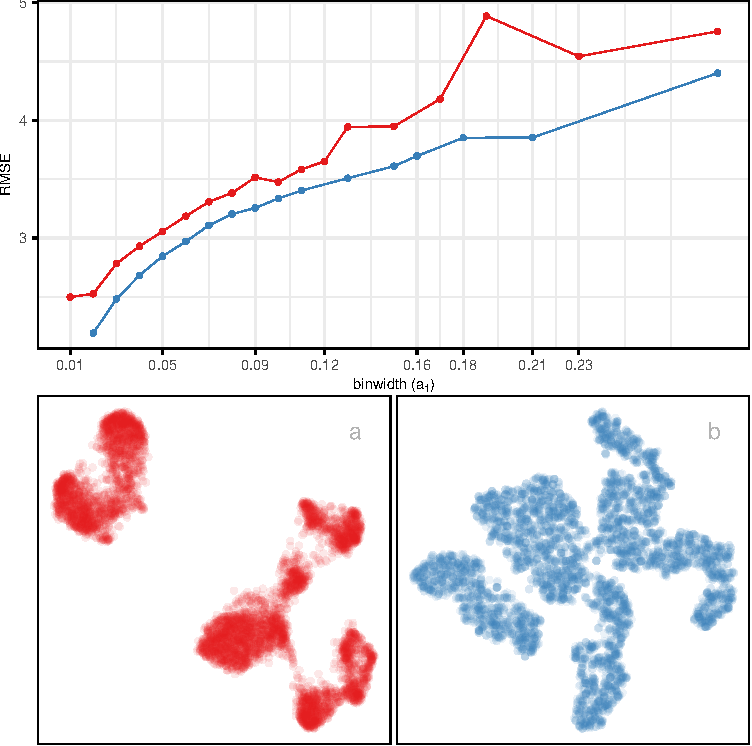
\includegraphics[width=1\linewidth,height=\textheight,keepaspectratio]{appendix_files/figure-pdf/fig-pbmc-mse-umap-1.pdf}

}

\caption{\label{fig-pbmc-mse-umap}Assessing which of the two layouts
with UMAP and tSNE with different hyper-parameter setting (n\_neighbors:
\(30\), min\_dist: \(0.3\) (red); n\_neighbors: \(30\) (blue)) on the
PBMC data is the better representation using RMSE for varying binwidth
(\(a_1\)). Colour used for the lines and points in the top plot and in
the scatterplots represents UMAP and tSNE layouts (a, b). Of the two,
layout b is optimal across all binwidths making it the best choice.}

\end{figure}%

\begin{figure}[H]

\centering{

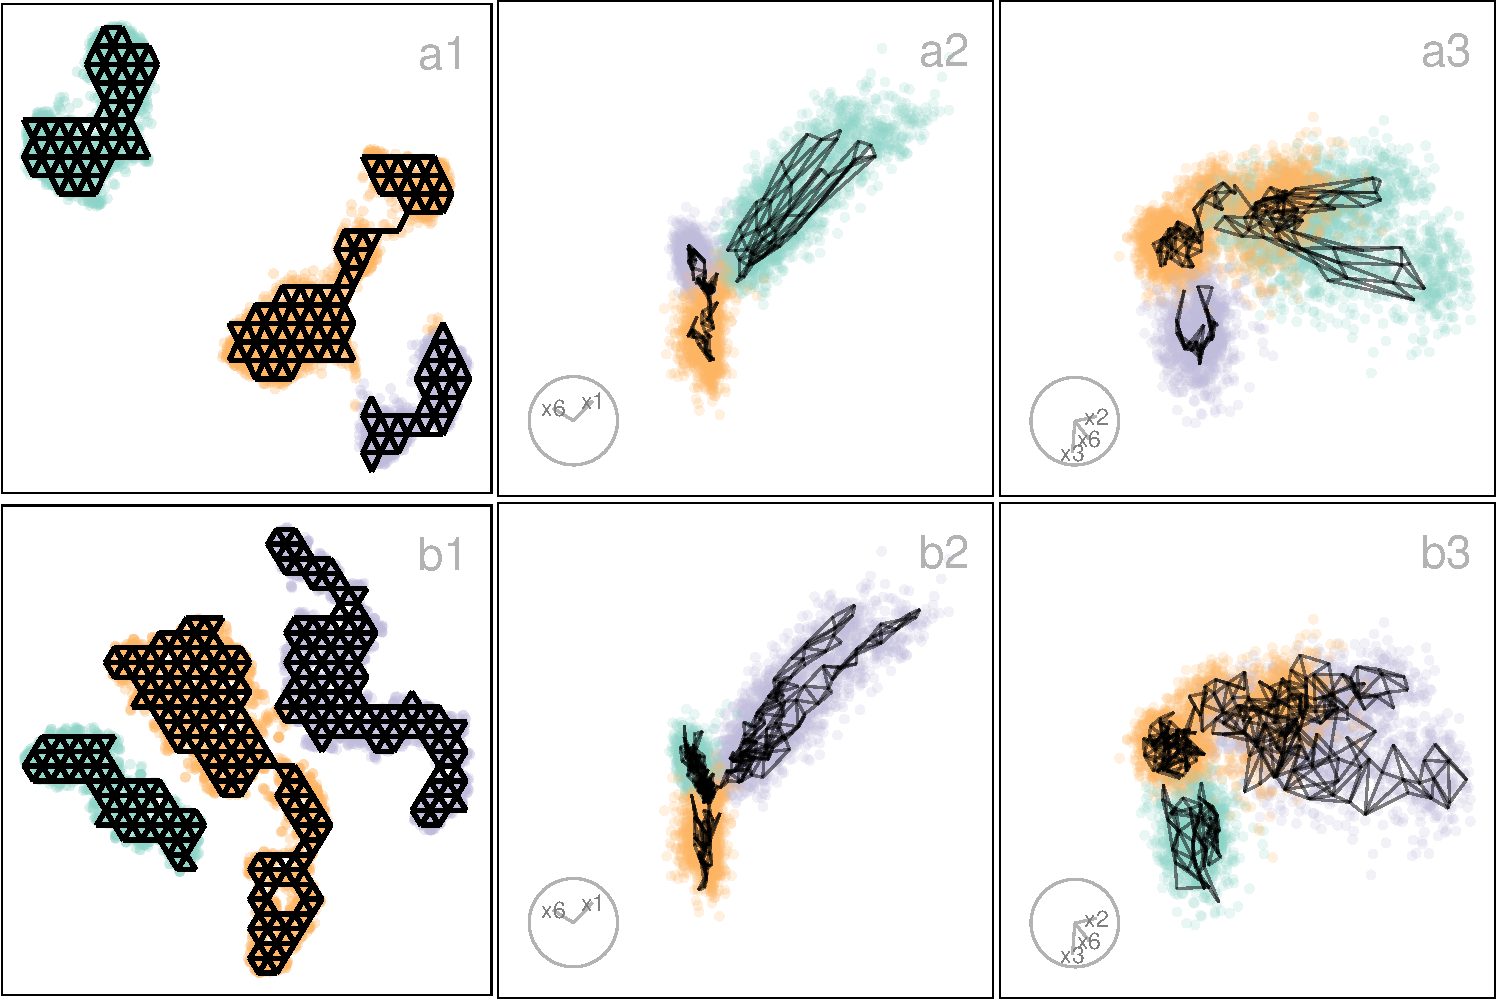
\includegraphics[width=0.9\linewidth,height=\textheight,keepaspectratio]{appendix_files/figure-pdf/fig-model-pbmc-author-proj-1.pdf}

}

\caption{\label{fig-model-pbmc-author-proj}Compare the published \gD{}
layout (Figure~\ref{fig-pbmc-mse-umap} a) and the \gD{} layout selected
(Figure~\ref{fig-pbmc-mse-umap} b) by MSE plot
(Figure~\ref{fig-pbmc-mse-umap}) from tSNE and UMAP with default
hyper-parameters. The PBMC3k data (\(n =  5858\)) has three clusters in
\(9\text{-}D\), where three clusters are close. Two \gD{} projection
from a tour on \(9\text{-}D\) of the model fit with
Figure~\ref{fig-pbmc-mse-umap} a (\(a_1 = 0.06\),
\(b = 616/86 (22, 28)\)) shows three-well separated clusters with big
separations. On the other hand, the model fit with
Figure~\ref{fig-pbmc-mse-umap} b (\(a_1 = 0.06\),
\(b = 704/227 (22, 32)\)) shows three-well separated clusters with small
separations. Therefore, Figure~\ref{fig-pbmc-mse-umap} b is more
reasonable than Figure~\ref{fig-pbmc-mse-umap} a. Videos of the
langevitour animations are available at
\url{https://youtu.be/0cKX_HG_n0k} and
\url{https://youtu.be/KhJvsRtaX04} respectively.}

\end{figure}%


  \bibliography{paper.bib}



\end{document}
